As the application launches, the first screen the user sees, in both the Google Glass version and the smartphone version, is the camera screen. The user must, in order to proceed further within the application, scan a QR code. Scanning a QR code is done by positioning the device's camera such that the QR code can be seen on screen, as seen in Figure~\ref{glassDemoQR}. The user does not need to press any shutter button as the application automatically recognises the QR code pattern if seen on screen.%, as seen in Figure~\ref{}. The reasoning behind 

%	\begin{figure}[ht!]
%		\centering
%		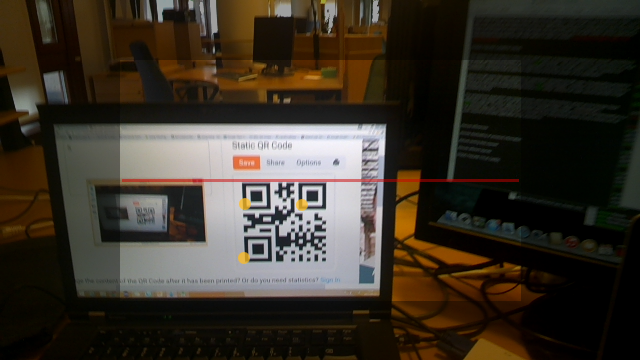
\includegraphics[width=110mm]{images/demo/qrCode}
%		\caption{todo bild behöver uppdateras}
%		\label{glassDemoQR}
%	\end{figure}
	
	\begin{figure}[ht!]
		\centering
    		\subfloat[The Google Glass application.]{{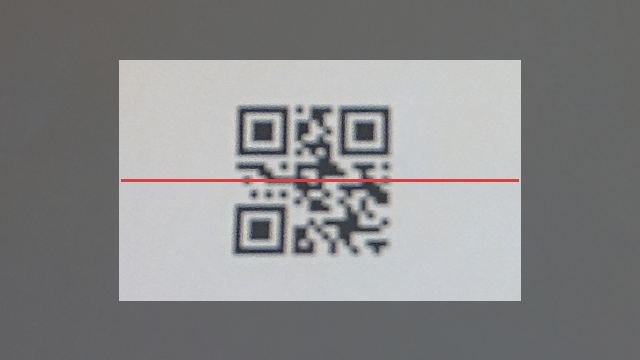
\includegraphics[width=70mm]{images/demo/qrCodeNew}}}
   		 \qquad
		\subfloat[The smartphone application.]{{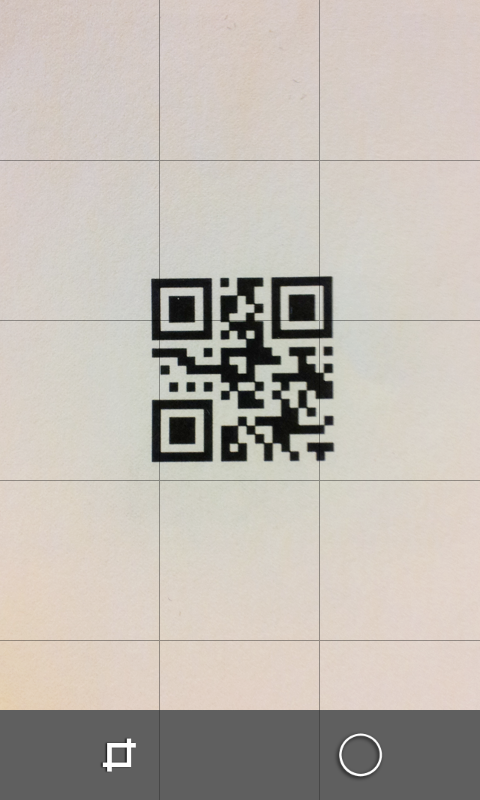
\includegraphics[width=70mm]{images/demo/smartphone/qrCodeNew}}}
   		 \qquad
		\caption{The application is scanning a QR code.}
		\label{glassDemoQR}
	\end{figure}

The reason for not providing a menu on the start screen or even requiring the user to press a shutter button is because the application should be simple, easy to use and focus on what is important. Since the the first step when using the application is to scan a QR code in order to receive the necessary information on the specific product, the scanning is also the main focus on the first screen of the application.

When the QR code has been scanned the application decodes the QR code. The decoding process is handled by the Zebra Crossing (ZXing) library~\cite{zxing}. ZXing is an open source barcode image processing library which uses the default QR code reader installed on the device.

The smartphone application was based directly on the ZXing library, where as the Google Glass application was based on a port of the ZXing library to Google Glass, called BardcodeEye~\cite{barcodeEye}. The main difference between ZXing and BarcodeEye is the fact that BarcodeEye is an example application ready to be run on Google Glass, in contrast to the ZXing library which is a library and as such needs to be attached to a runnable application.

The BarcodeEye application for Google Glass is however a bare bone application, used as an example and introduction as to how ZXing may be implemented in an application for Google Glass. BarcodeEye displays the decoded information from the QR code and also gives the user the option to search the internet using the information previously decoded from the QR code.

As the QR code is meant to encode only a product ID, and the application will then use the ID to download the product information (rather than having all of the instructions encoded directly in the QR code), the BarcodeEye application had to be modified. The first modification was on the graphical layout of the BarcodeEye application. The change of layout was mostly done due to the fact that the BarcodeEye application only displayed plain text, not taking in to account for instance a mix of image and text.

In order to display information BarcodeEye used the deprecated class \texttt{Card}, as seen in Listing~\ref{listingDeprecated}. The application now instead uses the \texttt{CardBuilder} class, as seen in Listing~\ref{listingRecommended}, as recommended by Google~\cite{googleCard}. The \texttt{CardBuilder} class allows users to input a desired layout style as an argument to the constructor of the \texttt{CardBuilder} class. With the \texttt{Card} class, developers could (in a separate method call) set where on the card the image would appear. For instance, in order to create a columns card, as seen in Figure~\ref{glassDemoComponentColumn}, the code would look as the code in Listing~\ref{listingDeprecated}. Using the recommended \texttt{CardBuilder} class instead would look as the code in Listing~\ref{listingRecommended}. With \texttt{CardBuilder} developers can now use default layouts, enabling more consistent application design across Google Glass applications. If a developer wishes to use a custom layout instead, the developer can simply use the custom layout as input to the \texttt{CardBuilder} class' constructor instead.

\begin{lstlisting}[language=Java, caption={Instancing of the deprecated class Card}, label=listingDeprecated]
Card card = new Card(context);
card.setImageLayout(Card.ImageLayout.LEFT);
\end{lstlisting}

\begin{lstlisting}[language=Java, caption={Instancing of the recommended class CardBuilder}, label=listingRecommended]
CardBuilder cardBuilder = new CardBuilder(context, CardBuilder.Layout.COLUMNS);
\end{lstlisting}

Since the smartphone application also used the ZXing library, but without any pre-existing application, no changes similar to those made to the Google Glass application had to be made for the smartphone application. Instead the smartphone application was built from the beginning to make use of the ZXing library's functionality, similar to how the ZXing library was integrated in the base Google Glass application.

The Google Glass application and the smartphone application are similar in how they are built. However, they look a bit different from each other, as seen in Figure~\ref{umlDiagrams}, which shows a UML diagram over the slide view part of the respective applications. The Google Glass version has a few extra classes involving result processors.

The result processors come from the base version of the Google Glass application, where more specific information was expected to be encoded in the QR code. For instance, the base version contained a ISBN processor for books, which was not needed in the application described in this dissertation. In the base version the \texttt{ResultProcessorFactory} returned a specific result processor depending on which information was to be processed. However, in the application only the \texttt{TextResultProcessor} is used and as such also the only remaining \texttt{ResultProcessor}. The Google Glass version should be rebuilt so that the \texttt{DownloadProductTask} replaces all three of the result processor classes. However, such refactoring has not been done at this point. 

%[TODO UML DIAGRAM ref(uml)]

	\begin{figure}[ht!]
		\centering
    		\subfloat[Google Glass.]{{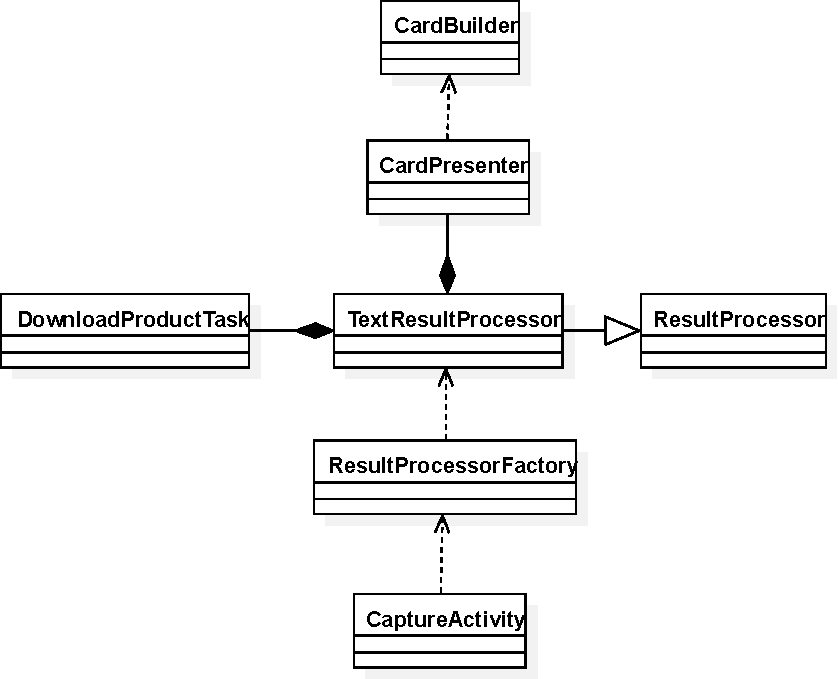
\includegraphics[width=100mm]{images/classDiagram/GoogleGlassClassDiagram.pdf}}}
   		 \qquad
		\subfloat[Smartphone.]{{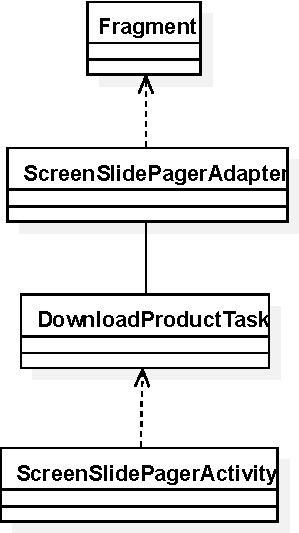
\includegraphics[width=30mm]{images/classDiagram/SmartphoneClassDiagram.pdf}}}
   		 \qquad
		\caption{UML diagrams.}
		\label{umlDiagrams}
	\end{figure}
	
In Figure~\ref{umlDiagrams}~(b) the class \texttt{Fragment} can be seen. The \texttt{Fragment} class is actually only an interface which is implemented by several other classes, however the UML diagram in Figure~\ref{umlDiagrams}~(b) has been simplified as all classes inheriting the \texttt{Fragment} class essentially do what the \texttt{CardBuilder} class in the Google Glass application does, which is setting up the specific layout of the slide. In the smartphone application there is a class for each different layout, in comparison to the Google Glass application where the \texttt{cardBuilder} class handles the layout through argument, as seen in Listing~\ref{listingRecommended}. As such another potential refactor which could be made is to create a general class that inherits the \texttt{Fragment} class and which takes the desired layout as an argument, similar to the \texttt{CardBuilder} class in the Google Glass application. Since the \texttt{CardBuilder} class is a Google Glass specific feature the \texttt{CardBuilder} class could not be used in the smartphone application.

%discuss differences (classes exclusive to the smartphone application and GG application respectivly)

%discuss downloading of product information

Having scanned and decoded a QR code the decoded information is then used to download information about the specific product. The downloaded information contains the product name, as well as the necessary components and instructions for assembling the product. The components and instructions may be represented by text, images or both. 

The way the download process uses the decoded product ID is by concatenating the product ID with a URL adress, which connects to a database containing all necessary information regarding the specific product. The download process was done using a \texttt{AsyncTask}. An AsyncTask is a class which performs operations in the background on a different thread than the user interface, such that the user interface is not frozen when the download process is taking place~\cite{asyncTask}.

In the Google Glass application a loading bar pops up at the bottom of the screen when information is being downloaded, as seen in Figure~\ref{downloadLoading}~(a), indicating that the application is loading. Google calls the bar an ``Indeterminate Slider'', as the the class used in implementation is the same as for a regular Slider~\cite{indeterminateSlide}. A similar animation was added to the smartphone application. However, in contrast to the Google Glass application's loading bar the smartphone application instead displays a spinning wheel at the center of the screen, seen in Figure~\ref{downloadLoading}~(a), indicating that the application is loading. The spinning wheel is implemented by the \texttt{ProgressDialog} class~\cite{loadingWheel}.

In both cases of loading animation the animation is started in the \texttt{AsyncTask}, just before the download begins. The loading animation stops when the \texttt{AsyncTask} has finished downloading the product information.

%However, such a spinner was not implemented in the Google Glass application. The reason for not implementing such a download spinner in the Google Glass application was because the AsyncTask, in order to display anything during the execution of the AsyncTask, requires access to a \texttt{Context} instance. A context comes from an activity in the android application, but in the Google Glass application the download process i taking place in between the scanning activity and the presenting activity. As such, the loading spinner 

	\begin{figure}[ht!]
		\centering
    		\subfloat[The Google Glass application]{{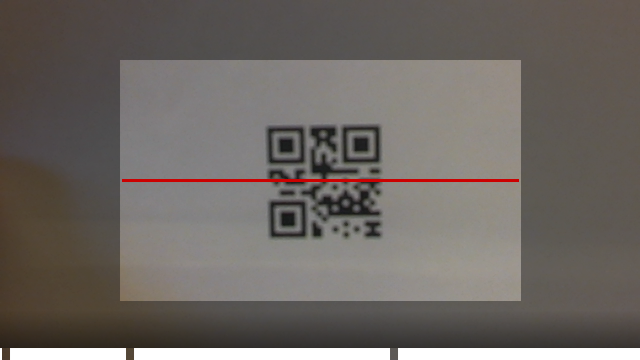
\includegraphics[width=70mm]{images/demo/loadingBar}}}
   		 \qquad
		\subfloat[The smartphone application.]{{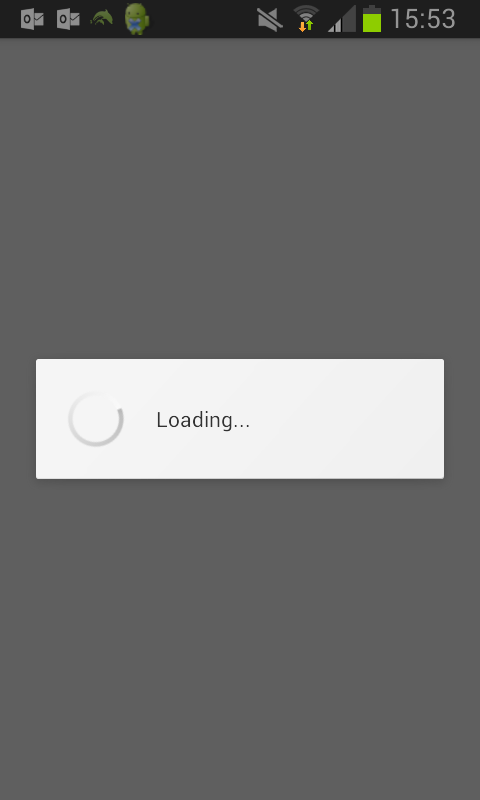
\includegraphics[width=70mm]{images/demo/smartphone/loadingSpinner}}}
   		 \qquad
		\caption{The loading screens.}
		\label{downloadLoading}
	\end{figure}

The download process also includes the creation and initialisation an instance of the \texttt{Products} class. The instance contains the name of the product and an image of the product as the product will look when the user is finished assembling all the components (the existence of an image is dependent on whether there was an image of the product stored in the database or not).

The Products class instance will also contain a list of components as well as a list of instructions. Both components and instructions are classes themselves. Similar to the \texttt{Products} class, instances of both the \texttt{Components} class and the \texttt{Instructions} class will contain a string and potentially an image, depending on whether there is an image stored in the database or not. In the case of components the string attribute will contain the name of the component, in contrast to instances of the \texttt{Instructions} class where the string instead will contain the instruction itself.

When the downloaded information is being displayed, the first screen the user sees contains the product name as well as an image of the product (if an image existed in the database). In the example case, lego parts are to be assembled in order to construct the so called ``Space Pirate'', seen in Figure~\ref{glassDemoRaw}.

	\begin{figure}[ht!]
		\centering
		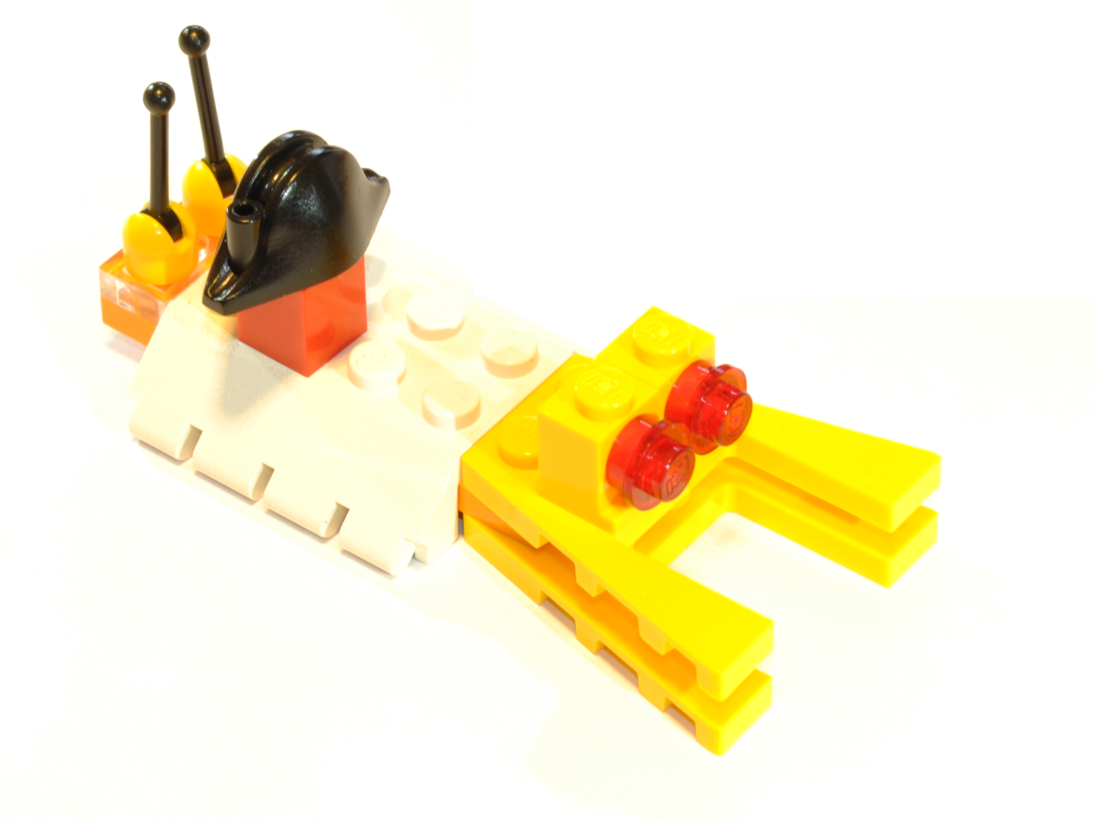
\includegraphics[width=90mm]{images/rawImages/BILD_6}
		\caption{The product.}
		\label{glassDemoRaw}
	\end{figure}

The first information the user sees displayed on screen after the QR code has been scanned and the information has been downloaded is the title page for the Space Pirate product, seen in Figure~\ref{glassDemoTitleCard}.

%	\begin{figure}[H]%ht!]
%		\centering
%		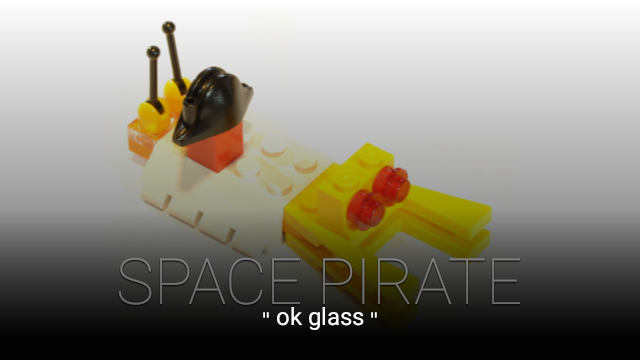
\includegraphics[width=110mm]{images/demo/titleCard}
%		\caption{The title card of the demo application.}
%		\label{glassDemoTitleCard}
%	\end{figure}
	
	\begin{figure}[ht!]
		\centering
    		\subfloat[The Google Glass application]{{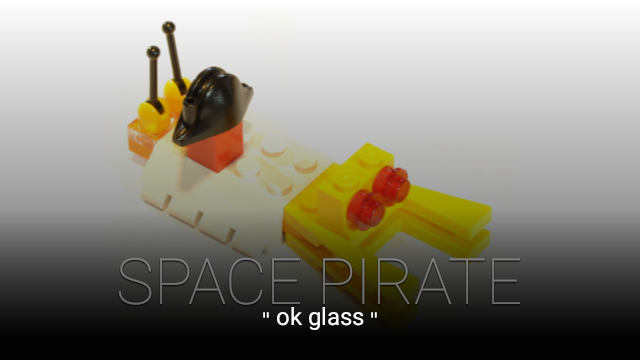
\includegraphics[width=70mm]{images/demo/titleCard}}}
   		 \qquad
		\subfloat[The smartphone application.]{{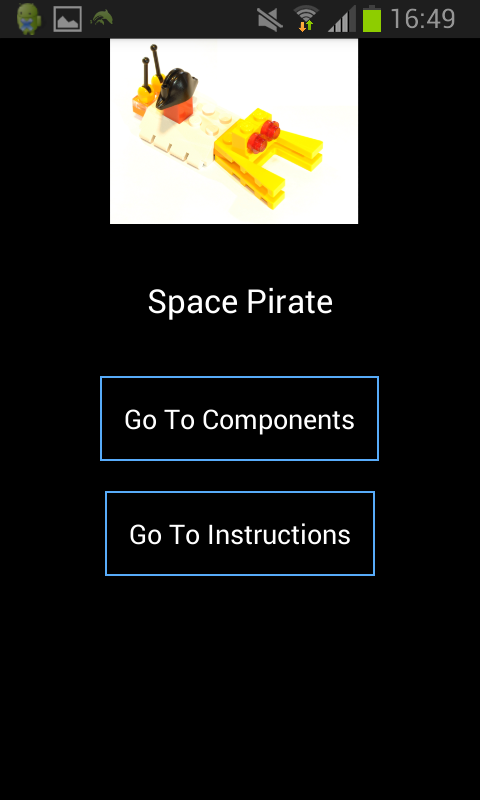
\includegraphics[width=70mm]{images/demo/smartphone/titleCard}}}
   		 \qquad
		\caption{The title card of the application.}
		\label{glassDemoTitleCard}
	\end{figure}
	
The next slide in line after the title slide is the first slide containing information on the components necessary for constructing the specific product. Each component has its own slide as the component may contain an image as well as the name of the component. Examples of a component described in only text can been seen in Figure~\ref{glassDemoComponentText} and examples of when the component has been described with both text and image can be seen in Figure~\ref{glassDemoComponentColumn}.

As seen in Figure~\ref{glassDemoComponentText} the text in the Google Glass application is larger than the text in the smartphone application. The difference in size is due to the automatic scaling in the Google Glass application. If the text in the Google Glass application were to cover the entire screen the text size would automatically be downscaled. In the smartphone application, however, the text is always the same size. The size of the text in the smartphone application was set to \texttt{MEDIUM} which is one of the three different default sizes of text used in android applications. The footer text, which in Figure~\ref{glassDemoComponentText} says ``Components'', as well as ``1/4'', is of the default size \texttt{SMALL}. In Figure~\ref{glassDemoTitleCard} the size of the product name text is of the default size \texttt{LARGE}. The reason behind the choice of the different text sizes is to keep the smartphone application similar to the Google Glass application, making the comparison of the two version easier.
%	\begin{figure}[H]%ht!]
%		\centering
%		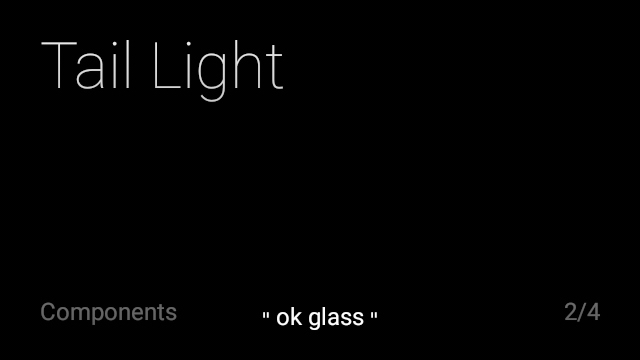
\includegraphics[width=110mm]{images/demo/componentText}
%		\caption{A component slide from the demo application.}
%		\label{glassDemoComponentText}
%	\end{figure}

		\begin{figure}[ht!]
		\centering
    		\subfloat[The Google Glass application]{{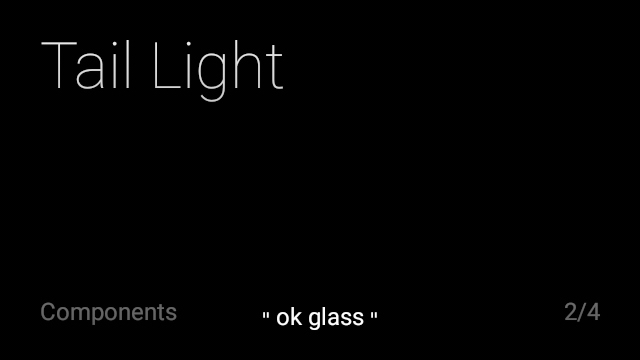
\includegraphics[width=70mm]{images/demo/componentText}}}
   		 \qquad
		\subfloat[The smartphone application.]{{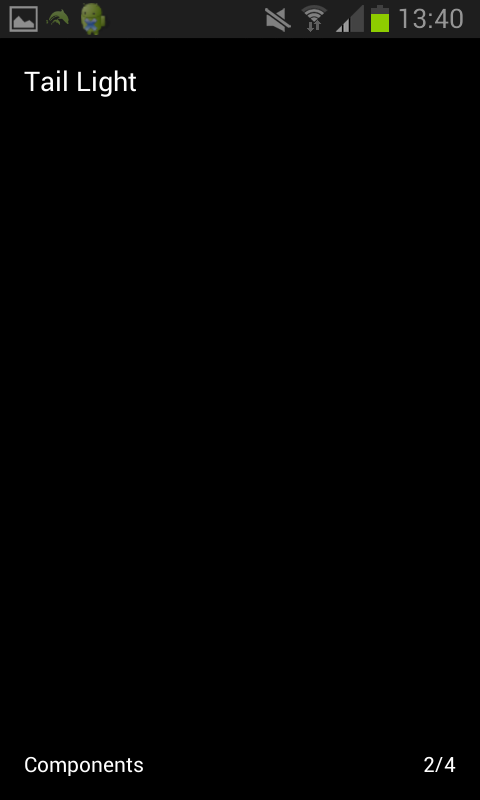
\includegraphics[width=70mm]{images/demo/smartphone/componentText}}}
   		 \qquad
		\caption{A component slide from the application.}
		\label{glassDemoComponentText}
	\end{figure}

%	\begin{figure}[H]%ht!]
%		\centering
%		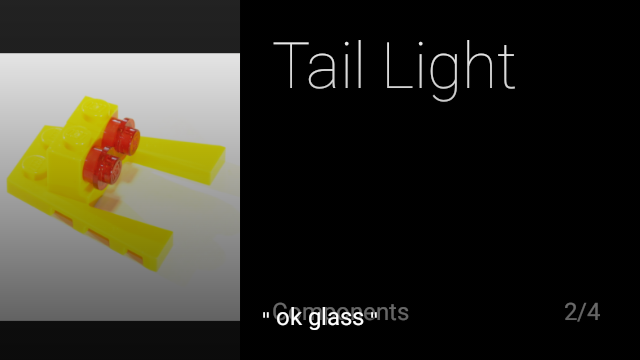
\includegraphics[width=110mm]{images/demo/columnImage}
%		\caption{A component slide from the demo application.}
%		\label{glassDemoComponentColumn}
%	\end{figure}
	
	\begin{figure}[ht!]
		\centering
    		\subfloat[The Google Glass application]{{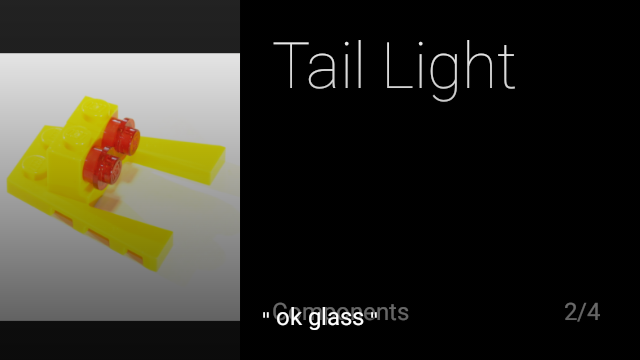
\includegraphics[width=70mm]{images/demo/columnImage}}}
   		 \qquad
		\subfloat[The smartphone application.]{{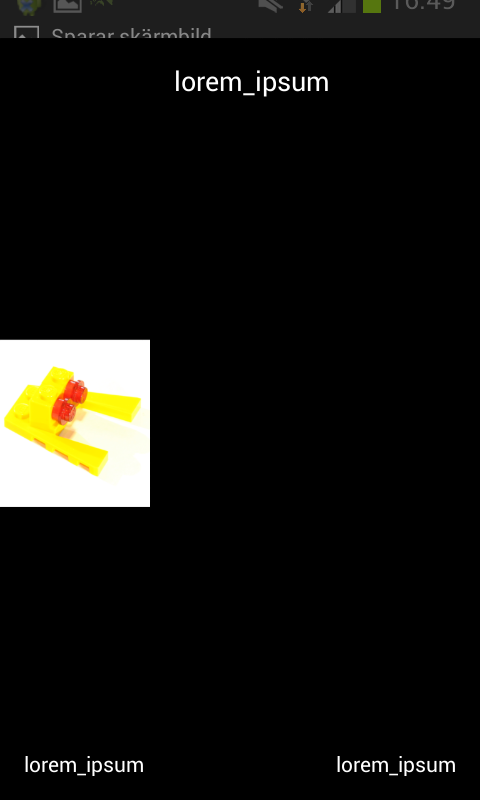
\includegraphics[width=70mm]{images/demo/smartphone/columnImage}}}
   		 \qquad
		\caption{A component slide from the application.}
		\label{glassDemoComponentColumn}
	\end{figure}

%	\begin{figure}[H]%ht!]
%		\centering
%		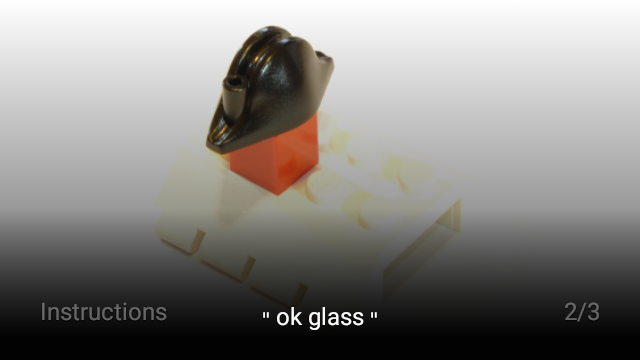
\includegraphics[width=110mm]{images/demo/instructionImage}
%		\caption{An instruction slide from the demo application.}
%		\label{glassDemoInstructionImage}
%	\end{figure}

The card design used for the component slide contains only text, seen in Figure~\ref{glassDemoComponentText}, is the predefined \texttt{TEXT} layout, used in similar fashion to how the title card design was specified in Listing~\ref{listingRecommended}. A component slide may also contain an image as complement to text. The card design used for the component slide containing both text and image, seen in Figure~\ref{glassDemoComponentColumn} is the predefined \texttt{COLUMNS} layout, used in similar fashion to how the title card design was specified in Listing~\ref{listingRecommended}

After all the component slides follow the instruction slides. These slides may also contain either text only or both text and an image, and these layouts are specified the same way as the component slides. However, an instruction slide may also consist of only an image, and no text at all. The reason for having an image only layout as a possible card layout for an instruction slide is because an instruction may be best described with an image. Describing the same instruction in text may take up more slides than the image, as the image will only take up one slide. A slide containing only an image and no text will also mean that the image will be shown in a larger scale than when using both text and an image. As such more detail can be shown and users may get a better understanding for how the components should be assembled.

As seen in Figure~\ref{glassDemoInstructionImage}, one instruction is described with only an image and no text. Since the placement of the components are important, and potentially hard to specify in text, an image may describe the placement better. Note also that the smartphone application still has room for text. Potentially the image in the smartphone application could be expanded, for instance by giving the user the ability to zoom by pinch. However, such a feature does not exist.

	\begin{figure}[ht!]
		\centering
    		\subfloat[The Google Glass application]{{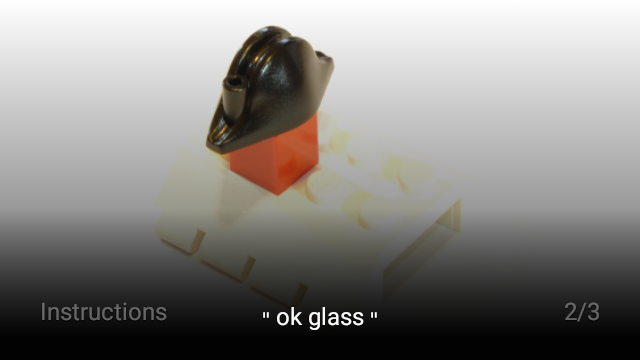
\includegraphics[width=70mm]{images/demo/instructionImage}}}
   		 \qquad
		\subfloat[The smartphone application.]{{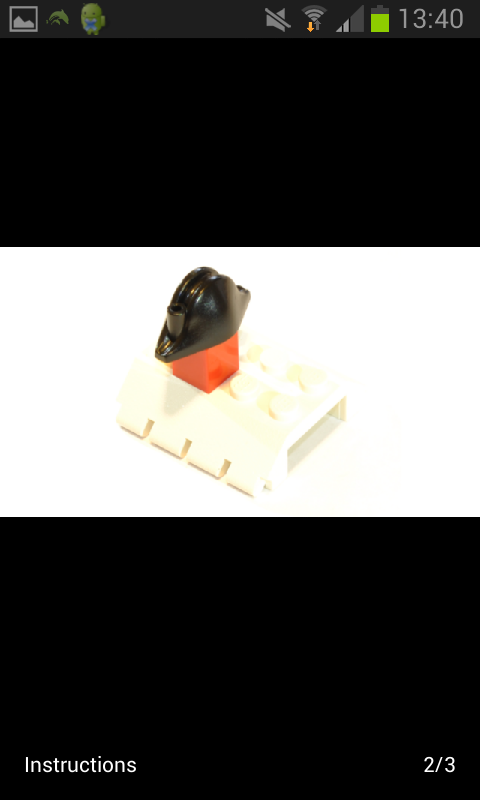
\includegraphics[width=70mm]{images/demo/smartphone/instructionImage}}}
   		 \qquad
		\caption{An instruction slide from the application.}
		\label{glassDemoInstructionImage}
	\end{figure}
	
The Google Glass application may be controlled by swiping across the Google Glass touchpad, but the Google Glass application may also be controlled using voice commands. The voice commands can be used as simple replacement for the touchpad, where users may swipe cards both backwards and forwards. However, using voice commands users may also ``jump'' in the application. By for instance saying ``ok glass, show components'' the application jumps to the first component slide, regardless of which slide the user is currently viewing. If the user is currently already viewing the first component slide nothing will happen. The voice command menu of the Google Glass application can be seen in Figure~\ref{glassDemoVoiceCommand}. Although the smartphone application does not have any voice command features the title slide contains buttons, as seen in Figure~\ref{glassDemoTitleCard}~(b) giving the user the ability to skip straight to the instructions is so desired.
	
	\begin{figure}[ht!]
		\centering
		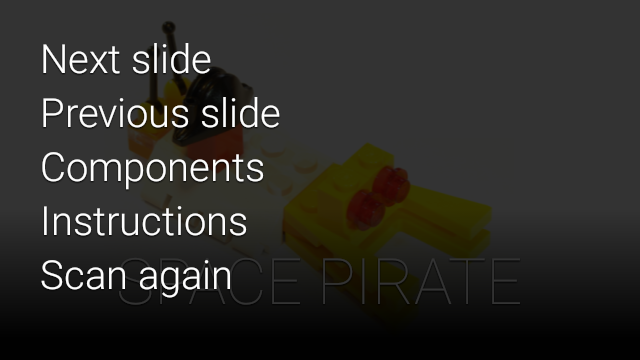
\includegraphics[width=90mm]{images/demo/glassVoiceCommand}
		\caption{The voice command menu.}
		\label{glassDemoVoiceCommand}
	\end{figure}

%discuss sorting into classes

%discuss different layouts

\subsection{Android Studio}
Since Google Glass runs Android as the operating system  todo API level 19, Glass Development Kit GDK

Both the smartphone application as well as the Google Glass application were developed in Android Studio~\cite{androidStudio}. Android Studio is a development environment developed by Google. Both applications were initially being developed in Eclipse~\cite{eclipse}, however development soon shifted to Android Studio as Android Studio is now the official integrated development environment (IDE) for Android~\cite{androidIDE}. The change was made without complications as Android Studio contains an import feature enabling developers to import projects previously not developed in Android Studio~\cite{androidIDE}.
%[TODO why Android Studio]

%\subsection{ZXing}
%The application was built upon the open-source barcode image processing library, Zebra Crossing (ZXing). 
%[TODO Vilka förändringar har gjorts]
% https://github.com/zxing/zxing/

%\subsubsection{BarcodeEye}
%The Google Glass application was built upon the Google Glass port of the ZXing library, known as BarcodeEye~\cite{barcodeEye}.% [TODO vilka förändringar har gjorts]%While a slideview was implemented in BarcodeEye already, the information displayed was static [todo, var den statisk]. The slideview consited of only two slides [todo code example of how it was static]. Mixing images with text was not possible either. Information also had to be encoded directly into the QR code and could not be downloaded by an encoded link.
% https://github.com/BarcodeEye/BarcodeEye

%\subsection{View Slider}


%\subsection{AsyncTask}

%Used for image, as well as product

%\subsection{Text Split}


\subsection{Card Layout}
Google provides developers with a set of predefined layouts for different types of cards, which were used in the Google Glass application and used as basis for the design of the different layouts for the slides in the smartphone application. The following predefined layouts were used in the implementation: ``Title'', ``Columns'', ``Text'' and ``Caption''. The Title layout was used for the first card of the slide view, which shows the product name as well as an image of the product as it is supposed to look when finished. 

	\begin{figure}[ht!]
		\centering
    		\subfloat[The title card layout.]{{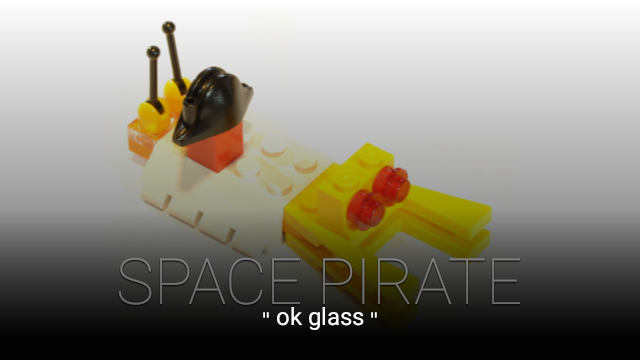
\includegraphics[width=70mm]{images/demo/titleCard}}}
   		 \qquad
		\subfloat[The column card layout.]{{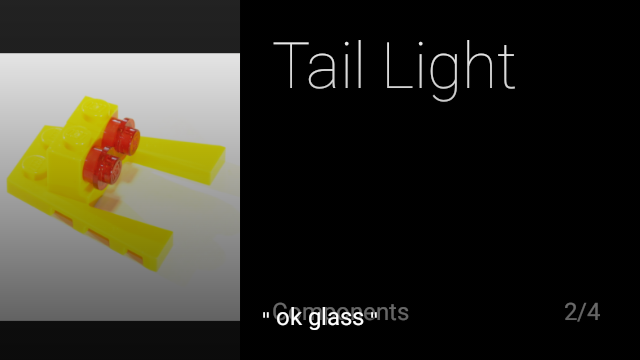
\includegraphics[width=70mm]{images/demo/columnImage}}}
   		 \qquad
    		\subfloat[The text card layout.]{{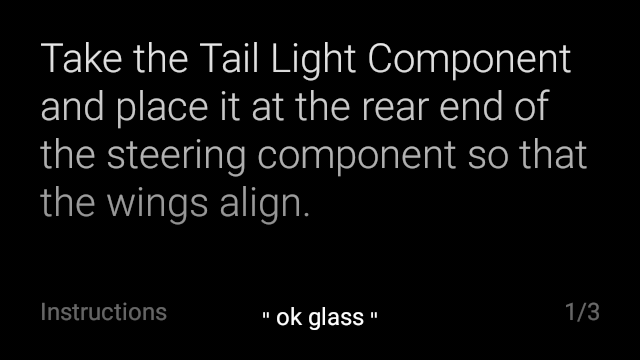
\includegraphics[width=70mm]{images/demo/instructionText}}}
    		\qquad
        		\subfloat[The image card layout.]{{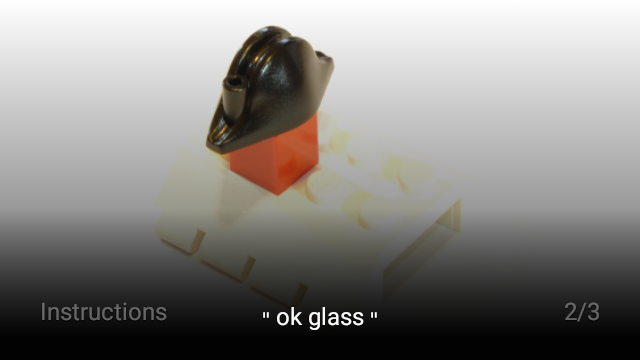
\includegraphics[width=70mm]{images/demo/instructionImage}}}
   		 \qquad
		\caption{The different layouts used within the Google Glass application.}
		\label{fig:cardLayout}
	\end{figure}

The Columns card layout, seen in Figure~\ref{fig:cardLayout}~(b) was used for when an instruction or component was to be presented with both text and an image. Since the Columns layout split the card, with an image to the left and text to the right, the Columns layout was the most reasonable choice when presenting both text and an image. An alternative would have been to display the text on top of the image, the image could potentially have been hidden behind a larger amount of text. 

Such a layout design was instead used for the title card as the amount of text being displayed is only the name of the product, and the image is only to give an idea of what the finished product will look like. The layout design where the text overlapped the image was called Title and can be seen in Figure~\ref{fig:cardLayout}~(a).

If the information, either a component or an instruction, were to be presented as text only, the Text layout, seen in Figure~\ref{fig:cardLayout}~(c) was used. The Text layout displayed dynamically sized text. In other words, if there was a lot of text being displayed the text would be resized to fit the screen.

If the card were to only contain an image and no text the Caption layout was used, seen in Figure~\ref{fig:cardLayout}~(d). The Caption layout is similar to the Title layout, but in contrast to the Title layout the Caption layout also has both a footer and a timestamp at the bottom of the card on the left and right side respectively. The Caption layout enables the use of an actual caption, however a caption is not necessary and neither is a caption used in the application as the Caption layout was used when no text was meant to be displayed (not counting the footer and the timestamp which appears on all cards except for the title card).

Using the predefined layouts in the implementation was easily achieved as the process consisted mostly of plug-and-play. The \texttt{CardBuilder} class constructor took the layout as an argument, as seen in Listing~\ref{cardBuilderPlugPlay}. When and instance of the \texttt{CardBuilder} class was created what remained was to simply input the necessary information, such as the instruction text. Setting an image was done slightly differently than written information as images were loaded in using a separate thread. As soon as the \texttt{CardBuilder} method \texttt{getView} was called the card was built with the information that had been input.

\begin{lstlisting}[language=Java, caption={Initialisation of the CardBuilder class}, label=cardBuilderPlugPlay]
CardBuilder cardBuilder = new CardBuilder(context, CardBuilder.Layout.COLUMNS)
	.setText(getText())
	.setFootNote(mFootNote)
	.setTimestamp(mTimeStamp);

cardBuilder = (new LoadImage(isTitleCard(), getByteArray()).doInBackground(cardBuilder));

return cardBuilder.getView();
\end{lstlisting}

%which standard layout were used, one non-standard

\subsection{Voice Commands}
The Google Glass application gives users the option to use voice commands in order to navigate the slides. The user opens the voice command menu by saying ``ok glass'' at any point in the application when ``ok glass'' is written at the bottom of the screen. The voice command feature is available at all times except when the camera is active. In other words the voice commands are unavailable when the application is waiting to scan a QR code.

The voice command menu contains the following options.

\begin{itemize}
	\item \textbf{Show next slide}
	
	The application scrolls to the next slide. If the current slide is the last slide, and in other words no other slides are following, the application does nothing.
	\item \textbf{Show previous slide}
	
	The application scrolls to the previous slide. If the current slide is the first slide, and in other words no other slides are sits before it, the application does nothing.
	\item \textbf{Show components}
	
	The application scrolls to the first slide showing information on a component. If the user is currently on the first slide showing information on a component the application does nothing. 
	\item \textbf{Show instructions}
	
	The application scrolls to the first slide showing an instruction. If the user is currently on the first slide showing an instruction the application does nothing.
	\item \textbf{Scan again}
	
	The application launches the camera and expects the user to scan another QR code.
\end{itemize}

Implementing voice command in the Google Glass application is done by following Google's step-by-step guide on how to implement voice commands in Goole Glass applications~\cite{howToVoiceInput}. Listing~\ref{voiceCommandXML} shows the resulting XML which gives the voice commands used in the application. Using contextual voice commands means that ``ok glass'' is displayed at the bottom of the screen at all times when voice commands are available. ``ok glass'' also comes with a black overlay, seen for instance in Figure~{fig:cardLayout}, which is transparent yet darkens the slides a bit, especially near the bottom of the slides where ``ok glass'' appears. Although the dark overlay could potentially distort the slides a bit, especially when the slide contains only an image, it was as of implementing the voice command feature not possible to alter the ``ok glass'' overlay in any way~\cite{voiceCommandCustom1, voiceCommandCustom2}. The dark overlay does however ensure that ``ok glass'' is always visible, no matter what the background image look like.

\begin{lstlisting}[language=XML, caption={The voice command menu XML file}, label=voiceCommandXML]
<menu xmlns:android="http://schemas.android.com/apk/res/android">
	<item
		android:id="@+id/next_menu_item"
		android:title="Show next slide" >
	</item>
	<item
		android:id="@+id/previous_menu_item"
		android:title="Show previous slide" >
	</item>
	<item
		android:id="@+id/components_menu_item"
		android:title="Show components" >
	</item>
	<item
		android:id="@+id/instructions_menu_item"
		android:title="Show instructions" >
	</item>
	<item
		android:id="@+id/scan_menu_item"
		android:title="Scan again" >
	</item>
</menu>
\end{lstlisting}

Although none of the voice commands have been sent in for official approval by Google most of the voice commands follows the design guidelines provided by Google. As seen in Table~\ref{tab:voiceCommandCheckTableChecked} 11 och the 15 voice command guidelines provided by Google has been followed. However, some of the guidelines has been applied to some or most of the voice command used within the application, and not all. For instance ``Show components'' does not follow the first guideline of the voice command checklist. ``Show components'' is however still a part of the application as ``Show components'' is a key feature of the application.

	\begin{table}[ht!]
    		\caption{Voice Command Checklist~\cite{glassVoiceChecklist}.} \label{tab:voiceCommandCheckTableChecked}
		\centering \begin{tabularx}{\textwidth}{l|X|l} \hline
		 & \textbf{Guideline} & \textbf{Acheived} \\ \hline \hline
       
1	&	Is general enough to apply to multiple Glassware, but still has a clear purpose		&	Yes		\\ \hline
2	&	Is colloquial and can explain Glass features in a conversation					&	Yes		\\ \hline
3	&	Is comfortable to say in public											&	Yes		\\ \hline
4	&	Brings the user from intent to action as quickly as possible					&	Yes		\\ \hline
5	&	Avoids brand words													&	Yes		\\ \hline
6	&	Is long enough to ensure high recognition quality (at least three syllables)			&	Yes		\\ \hline
7	&	Fits on a single line													&	Yes		\\ \hline
8	&	Does not sound similar to existing commands								&	Yes		\\ \hline
9	&	Does not require immediate interactivity in Mirror API Glassware.				&	Yes		\\ \hline
10	&	Has an imperative verb with an object									&	Yes		\\ \hline
11	&	Uses articles when possible											&	No		\\ \hline
12	&	Uses definite articles only when the object is definite							&	No		\\ \hline
13	&	Uses ``this'' when there is only one relevant instance of the object				&	No		\\ \hline
14	&	Uses me and my when appropriate										&	No		\\ \hline
15	&	Refers to Glass as the subject carrying out the action						&	Yes		\\ \hline
		
		\end{tabularx}
	\end{table}

The reason for not following guidelines 11--14 is because they would make the voice commands longer. As the voice commands may potentially be said often while using the application, as the user may proceed through the slides quite fast, shorter voice commands makes for more comfortable use. As the voice commands still follows guideline 6 the voice commands were deemed to be long enough to still ensure high recognition quality.

\subsection{Test Cases}
%The following section describes how the tests were set up and carried out.
%
%\subsubsection{Experimental Setup}
The tests were carried out using an optical bench to guarantee scientific accuracy. The experimental setup contained an optical bench, with a screen holder at the zero point, where the QR code was positioned. The device being tested, Google Glass or smartphone, was then positioned at the specified mark on the optical bench using a clamp and pointed towards the QR code. See Figure~\ref{experimentalSetup} for a better understanding of the experimental setup. 

As seen in Figure~\ref{experimentalSetup} Google Glass was mounted in such a way that the camera sat a bit closer to the QR code than where the clamp marked on the optical bench. In order to compensate for the slight misalignment the clamp was positioned a few centimeters back from the specified mark and as such not used to determine the distance to the QR code. Instead the camera on Google Glass was used to pinpoint the exact distance to the QR code, and the clamp was positioned in such a way that the camera on Google Glass was at the distance specified in each experiment. In other words, even though the clamp was not at the same distance to the QR code for the smartphone tests as for the Google Glass tests, the camera of each device was.

	\begin{figure}[H]%ht!]
		\centering
    		\subfloat[The experimental setup for Google Glass.]{{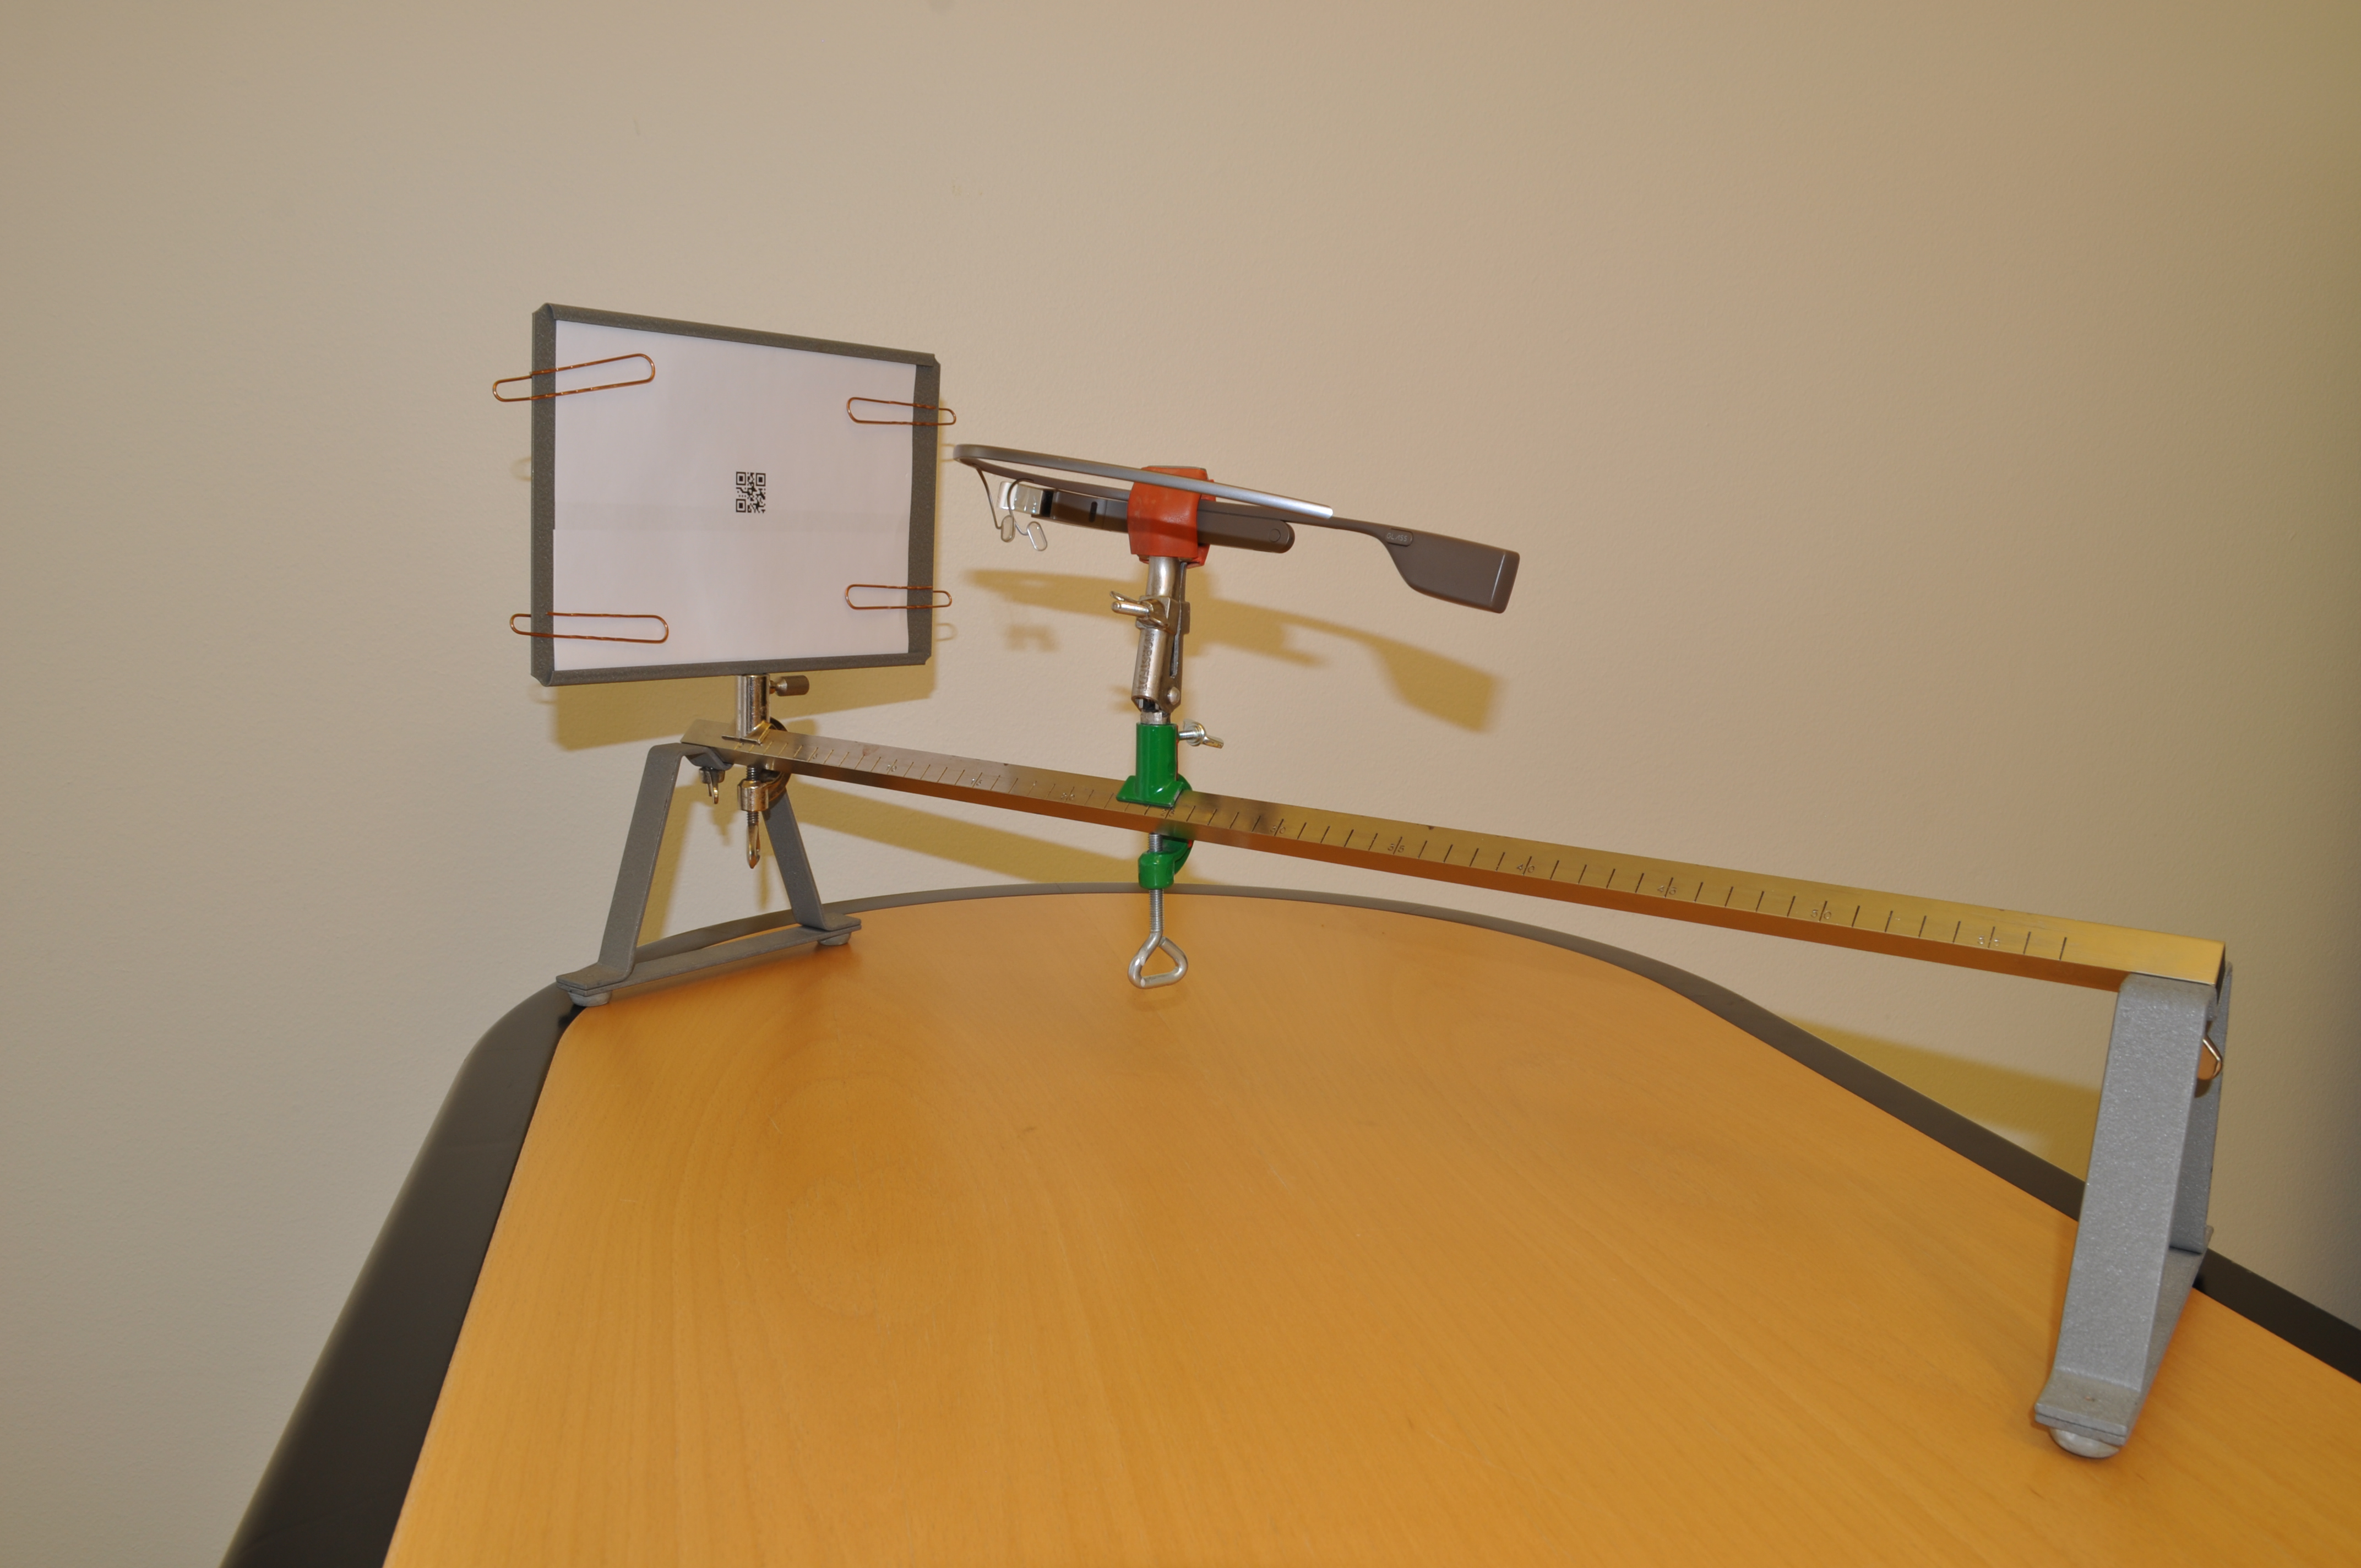
\includegraphics[width=70mm]{images/testSetupGlass}}}
   		 \qquad
		\subfloat[The experimental setup for Samsung Galaxy SII.]{{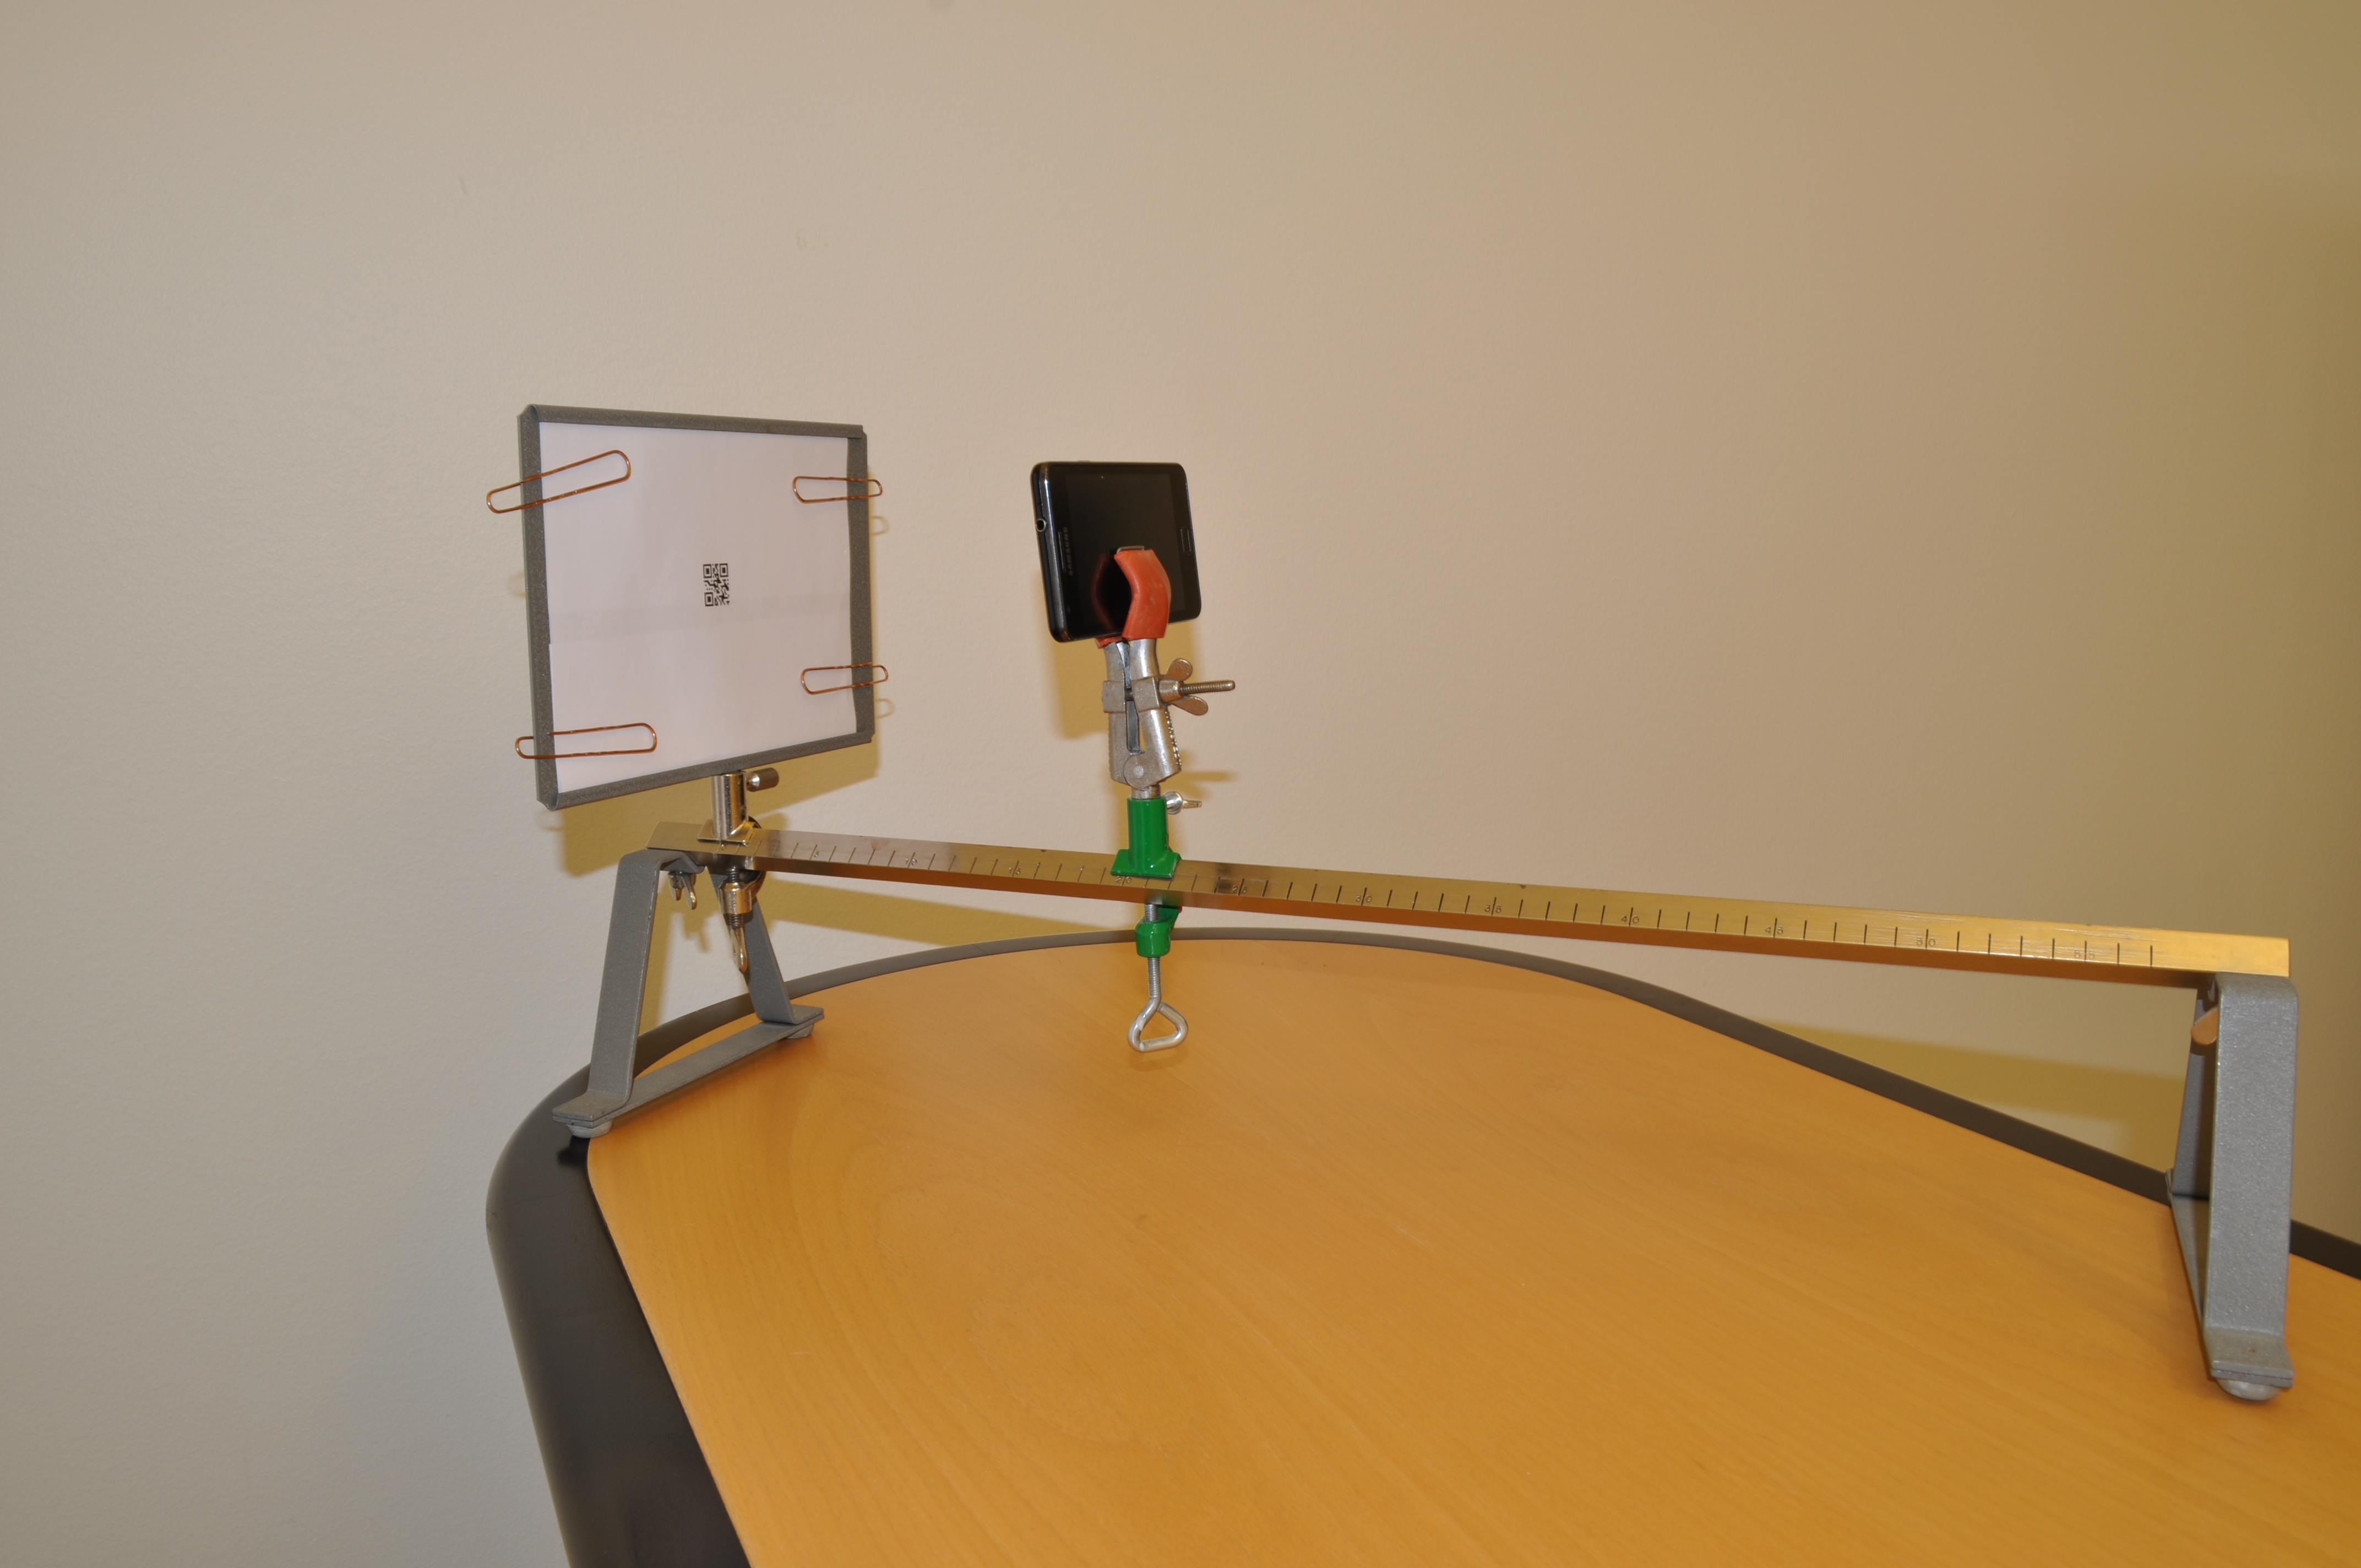
\includegraphics[width=70mm]{images/testSetupS2}}}
   		 \qquad
		\caption{The experimental setup.}
		\label{experimentalSetup}
	\end{figure}

Although not shown i Figure~\ref{experimentalSetup} each device was connected to a computer via a USB cable. The result time of each test was obtained from the log within Android Studio after each run, since when running an android application via Android Studio, log information may be obtained through the log within Android Studio.

In order to measure the time needed for the results of each test a specific class was built, called \texttt{Timer} (seen in Listing~\ref{timerClass}). The \texttt{Timer} class was built using the singleton design pattern. A singleton class is a class that can only be instanced once during the entire execution of an application. However the instance of a singleton class lives throughout the entire execution and may be accessed from anywhere in the application.

Using the singleton pattern meant that the timer could be started in one class, and stopped in another without having to pass the instance around, which could potentially affect the performance of each device.

\begin{lstlisting}[language=Java, caption={The Timer class}, label=timerClass]

public class Timer {
	private static Timer ourInstance = new Timer();
	public static Timer getInstance() { return ourInstance; }
	private Timer() {  }
	
	private boolean timerRunning = false;
	private Long startTime;
	private Long stopTime;
	
	public void startTimer() { 
		if(timerRunning) { Log.d("TIMER", "Timer already running"); }
		else 	{ startIme = System.nanoTime(); }
	}
	
	public void stopTimer() {
		if(!timerRunning) { Log.d("TIMER", "No timer running"); }
		else { stopTime = System.nanoTime()); }
	}
	
	private long getElapsedTime(int timerID) { return stopTime - startTime; }
	
	public void logElapsedTime(String information) {
		Log.d("TIMER", information + ": " + String.valueOf(getElapsedTime() + " nano seconds");
	}
}
\end{lstlisting}

\subsubsection{Text Length}
When evaluating the text length the text string used was not a predefined one, but rather a randomised one. The text was randomly generated using the distribution of characters in regular English text. One might argue that technical texts have a slightly different distribution of characters, but Google recommends developers to be personal when writing text meant to be displayed to the user~\cite{glassDesignStyle}. The text was also short enough to fit a smartphone screen and as such the difference using slightly different distribution of characters would not have any major effect on the results.

Listing~\ref{randomizer} shows how each character was randomly selected. \texttt{randchar} was called from within a for loop where the character was added to a string. The number of loops determined how long the text was going to be. The \texttt{doubleList} list contained the distribution of each character according the their distribution in the english language~\cite{englishTextStat} and the \texttt{alph} list contained all the individual characters, including whitespace. As a decimal number between zero and one was randomly selected a corresponding character was picked out based on the distribution of that character.

A recursive method located the corresponding character and returned the character back up to the calling method \texttt{randchar} which in turns returned the character to the for loop in which a string of random characters were collected.

\newpage
\begin{lstlisting}[language=Java, caption={The randomizer class}, label=randomizer]
public RandomizeEnglishText() {
	doubleList = new ArrayList<>();
	doubleList.add(0.0651738);					// A
	doubleList.add(doubleList.get(0) + 0.0124248);		// B
	doubleList.add(doubleList.get(1) + 0.0217339);		// C
		[...]
	doubleList.add(doubleList.get(23) + 0.0145984);	// Y
	doubleList.add(doubleList.get(24) + 0.0007836);	// Z
	doubleList.add(doubleList.get(25) + 0.1918182);	// _
	alph = Arrays.asList("a", "b", "c", "d", "e", "f", "g", "h", "i", "j", "k", "k", "m", "n", "o", "p", "q", "r", "s", "t", "u", "v", "w", "x", "y", "z", " ");
}
private double randfrom(double min, double max) {
	Random rand = new Random();
	double range = (max - min);
	return min + range * rand.nextDouble();
}
private String getChar(int pos, double rand) {
	return (rand <= doubleList.get(pos) || pos+1 <= alph.size()) ?
		alph.get(pos) :
		getChar(pos+1, rand);
}
public String randchar() {
	double rand = randfrom(0, 1);
	return getChar(0, rand);
}
\end{lstlisting}

\subsubsection{Distance to the QR Code}

Using the \texttt{Timer} class, seen in Listing~\ref{timerClass}, the elapsed time from the start of the application until the QR code was decoded was measured for each device. The test was performed 30 times for each device, with 3 different distances between the QR code and the device. Figure~\ref{projectmap} described the application functionality and this test measures steps 1 and 2 in Figure~\ref{projectmap}. The results of the test can be seen in detail in Appendix~\ref{app:results} but will also be presented in a smaller table with the average time. 
%in a table similar to Table~\ref{tab:distanceAverage}. 
Although the \texttt{Timer} class will give the elapsed time in nanoseconds the result will be presented in seconds in order to clearly show the significance of each time as small, nano seconds, differences between devices will not matter as much as seconds.

%	\begin{table}[ht!]
% 		\caption{Average time of registering a QR code with varying distance.} \label{tab:distanceAverage}
%		\centering \begin{tabularx}{\textwidth}{l|X|X|X} \hline
%		\textbf{Distance (dm)} & \textbf{Google Glass (sec)} & \textbf{Samsung Galaxy SII (sec)} & \textbf{Samsung Galaxy SIII (sec)} \\ \hline \hline
%       
%		1.0	&	&	&	\\ \hline
%		2.0	&	&	&	\\ \hline
%		3.0	&	&	&	\\ \hline
%		
%		\end{tabularx}
%	\end{table}

\subsubsection{Complexity of the QR Code}

Using the \texttt{Timer} class, seen in Listing~\ref{timerClass}, the elapsed time from the start of the application until the QR code was decoded was measured for each device. The test was performed 30 times for each device, with 3 different complexities of the QR code. Figure~\ref{projectmap} described the application functionality and this test measures steps 1 and 2 in Figure~\ref{projectmap}. The results of the test can be seen in detail in Appendix~\ref{app:results} but will also be presented in a smaller table with the average time.
% in a table similar to Table~\ref{tab:complexityAverage}. 
Although the \texttt{Timer} class will give the elapsed time in nano seconds the result will be presented in seconds in order to clearly show the significance of each time as small, nanoseconds, differences between devices will not matter as much as seconds. Figure~\ref{qrCodeComplex} shows the three different QR codes used for the complexity test.

	\begin{figure}[H]%ht!]
		\centering
    		\subfloat[1 encoded character.]{{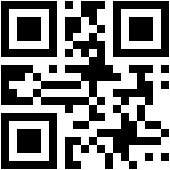
\includegraphics[width=20mm]{images/qrCodeComplex/1}}}
   		 \qquad
		\subfloat[50 encoded characters.]{{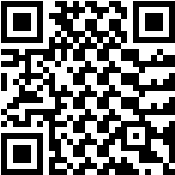
\includegraphics[width=20mm]{images/qrCodeComplex/50}}}
   		 \qquad
		\subfloat[100 encoded characters.]{{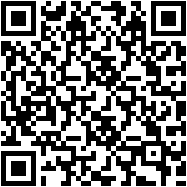
\includegraphics[width=20mm]{images/qrCodeComplex/100}}}
   		 \qquad
		\caption{The three different QR codes used in the complexity test.}
		\label{qrCodeComplex}
	\end{figure}

%	\begin{table}[H]%ht!]
%    		\caption{Average time of registering a QR code with varying density.} \label{tab:complexityAverage}
%		\centering \begin{tabularx}{\textwidth}{l|X|X|X} \hline
%		\textbf{Encoded Characters} & \textbf{Google Glass (sec)} & \textbf{Samsung Galaxy SII (sec)} & \textbf{Samsung Galaxy SIII (sec)} \\ \hline \hline
%       
%		1	&	&	&	\\ \hline
%		50	&	&	&	\\ \hline
%		100	&	&	&	\\ \hline
%		
%		\end{tabularx}
%	\end{table}

\subsubsection{Display Time}

Using the \texttt{Timer} class, seen in Listing~\ref{timerClass}, the elapsed time from the point that the product information had ben downloaded until the information was sent to the display was measured for each device. The test was performed 30 times for each device, with 3 different sizes of product information. Figure~\ref{projectmap} described the application functionality and this test measures steps 4 and 5 in Figure~\ref{projectmap}. The results of the test can be seen in detail in Appendix~\ref{app:results} but will also be presented in a smaller table with the average time. %in a table similar to Table~\ref{tab:averageDisplaySpeedGoogleGlass}. 
Although the \texttt{Timer} class will give the elapsed time in nanoseconds the result will be presented in seconds in order to clearly show the significance of each time as small, nano seconds, differences between devices will not matter as much as seconds.

%	\begin{table}[ht!]
%    		\caption{Average display time for Google Glass with varying information size.} \label{tab:averageDisplaySpeedGoogleGlass}
%		\centering \begin{tabularx}{\textwidth}{l|X|X|X} \hline
%		\textbf{Information Size (Bytes)} & \textbf{Google Glass (sec)}  & \textbf{Samsung Galaxy SII (sec)}  & \textbf{Samsung Galaxy SIII (sec)} \\ \hline \hline
%       
%		1 000		&	&	&	 \\ \hline
%		100 000		&	&	&	 \\ \hline
%		1 000 000		&	&	&	 \\ \hline
%
%		\end{tabularx}
%	\end{table}

\subsection{Summary}
\label{subsec:summary}
The application works in such a way that the first screen the user sees when launching the application, on both Google Glass and smartphones, is the camera screen. The user is then to position the device in such a way that the QR code may be scanned by the device's camera. The QR code contains a product ID for a specific product.

The user does not need to press any shutter button in order to scan the QR code. Instead the application will automatically recognise any QR code pattern that appears in the camera view, as well as scan the QR code. The reason for not implementing a start menu or any similar start screen, to show the user before the camera screen is displayed, is to, according to Google's design guidelines, maintain the focus on what the application is intended to do and to keep the application simple and easy to use.

Next the application will decode the QR code. The decoding process is done by the ZXing library, which is an open source  barcode image processing library. The QR code contains a product ID which is then used in the downloading process. The downloading process entails connecting to a database containing information about different products, and, by using the decoded product ID, retrieving the information on the specific product. 

The downloaded information contains the product name, as well as a list of components and the instructions necessary to assemble the product. All the information is then sorted in to respective classes and the information may be displayed to the user. When the product information is being downloaded a loading animation is displayed on screen. On Google Glass the loading information is a loading bar at the bottom of the screen, and in the smartphone application the loading animation is a spinning wheel.

When the download process has finished the information is displayed to the user in the form of a slide show. The first slide that is displayed to the user is the title slide. The title slide contains the name of the product as well as an image  (if an image existed in the database). Following the title slide are the component slides. Each component has their own slide due to the fact that a component may be described in both text and an image. 

After all the component slides follow the instruction slides. Similar to the components an instruction my be presented by text only or by both text and an image. In contrast to the components, however, instructions may also be presented with an image and no text. 

As Google provides developers of Google Glass applications with predefined layouts, these layouts were also used for the Google Glass application. The layouts used were ``Title'', ``Columns'', ``Text'' and ``Caption''. The predefined layouts were also used as basis for the layouts used in the smartphone application.

The Title layout is used for the title card. The Columns layout is used for the slides with both text and an image. The Text layout is used for the slides with text only. The Caption layout is used for the slides containing only an image. All layouts, except for the Title layout, also contain text at the bottom of the screen called ``footer'' and ``timestamp''. The footer contains information on whether the current slide is a component slide or an instruction slide. The timestamp contains information on which slide is currently being viewed.

While browsing through the slides in the Google Glass application, the user may also navigate using voice commands. The voice commands available in the Google Glass application are ``Show next slide'', ``Show previous slide'', ``Show components'', ``Show instructions'' and ``Scan again''.

Most of the voice commands follow 11 out of the 15 voice command guidelines provided by Google. For example, ``Show components'' does not follow the guidelines which state that ``Is general enough to apply to multiple Glassware, but still has a clear purpose''. ``Show components'' is a specific voice command and could potentially apply to multiple Google Glass applications, but not all.

While viewing the slides ``ok glass'' is shown at the bottom of the screen. ``ok glass'' indicates that voice commands are available and saying ``ok glass'' at that point brings up the voice command menu, showing all available voice commands. However, ``ok glass'' is also shown in combination with a dark, transparent overlay, which ensures ``ok glass'' is always visible no matter what image is shown on screen, but the dark overlay also means that any image shown is darkened by the overlay.

In terms of the testing performed on the application, the experimental setup consisted of an optical bench on which the QR code was positioned at the zero mark, and then each specific device was positioned so that the camera of each device was positioned according to the specifications of each test. Each test result was then obtained through a laptop with which each device was connected via a USB cable. The test results were printed out from a timer class, called \texttt{Timer}, which was implemented using the singleton design pattern, meaning that the class had only one global instance which could be accessed from anywhere within the application.

The test which did not require the experimental setup was the text length test. Instead the text length test was performed using a class which randomised English characters, which were then concatenated together to form a longer string.

Three other tests were performed using the experimental setup. In the first of these three tests the distance to the QR code was varied. In the second test the complexity of the QR code was varied. In the third and final test the size of the downloaded information was varied. Each of these tests were performed 30 times, for each device and each different specification, to ensure statistical significance.

%o   Implementation - Present your project implemetion in general
%o   Information - Give details here (possibly several sub-sections)
%o   Summary - for this chapter

% Mobile phone application
% Uses Zxing - library for QR code scanning [Link to gihub repository missing!!!]
% can display both text and images 
% 
% Google Glass Application
% Uses BarcodeEye - library for QR Code Scanning (port of Zxing for Google Glass) [Link to github repository missing!!!]
% Can display text, images still todo
% Much easier to add slides on Google Glass compared to Mobile Phone Application. Probably because Cards is standard interface for Google Glass (might also be because simple API, check CardPresenter!!!)
% Very difficult to add images since cards can't be changed after .getView() has been called
% Need to call .notifyViewChanged() but does not work anyway (yet) seems to only start the activity over which calls the execute method again if no check has been put in place